\documentclass[]{article}
\usepackage{lmodern}
\usepackage{amssymb,amsmath}
\usepackage{ifxetex,ifluatex}
\usepackage{fixltx2e} % provides \textsubscript
\ifnum 0\ifxetex 1\fi\ifluatex 1\fi=0 % if pdftex
  \usepackage[T1]{fontenc}
  \usepackage[utf8]{inputenc}
\else % if luatex or xelatex
  \ifxetex
    \usepackage{mathspec}
  \else
    \usepackage{fontspec}
  \fi
  \defaultfontfeatures{Ligatures=TeX,Scale=MatchLowercase}
\fi
% use upquote if available, for straight quotes in verbatim environments
\IfFileExists{upquote.sty}{\usepackage{upquote}}{}
% use microtype if available
\IfFileExists{microtype.sty}{%
\usepackage{microtype}
\UseMicrotypeSet[protrusion]{basicmath} % disable protrusion for tt fonts
}{}
\usepackage[margin=1in]{geometry}
\usepackage{hyperref}
\hypersetup{unicode=true,
            pdftitle={Stats Application},
            pdfauthor={Ben Kean},
            pdfborder={0 0 0},
            breaklinks=true}
\urlstyle{same}  % don't use monospace font for urls
\usepackage{graphicx,grffile}
\makeatletter
\def\maxwidth{\ifdim\Gin@nat@width>\linewidth\linewidth\else\Gin@nat@width\fi}
\def\maxheight{\ifdim\Gin@nat@height>\textheight\textheight\else\Gin@nat@height\fi}
\makeatother
% Scale images if necessary, so that they will not overflow the page
% margins by default, and it is still possible to overwrite the defaults
% using explicit options in \includegraphics[width, height, ...]{}
\setkeys{Gin}{width=\maxwidth,height=\maxheight,keepaspectratio}
\IfFileExists{parskip.sty}{%
\usepackage{parskip}
}{% else
\setlength{\parindent}{0pt}
\setlength{\parskip}{6pt plus 2pt minus 1pt}
}
\setlength{\emergencystretch}{3em}  % prevent overfull lines
\providecommand{\tightlist}{%
  \setlength{\itemsep}{0pt}\setlength{\parskip}{0pt}}
\setcounter{secnumdepth}{0}
% Redefines (sub)paragraphs to behave more like sections
\ifx\paragraph\undefined\else
\let\oldparagraph\paragraph
\renewcommand{\paragraph}[1]{\oldparagraph{#1}\mbox{}}
\fi
\ifx\subparagraph\undefined\else
\let\oldsubparagraph\subparagraph
\renewcommand{\subparagraph}[1]{\oldsubparagraph{#1}\mbox{}}
\fi

%%% Use protect on footnotes to avoid problems with footnotes in titles
\let\rmarkdownfootnote\footnote%
\def\footnote{\protect\rmarkdownfootnote}

%%% Change title format to be more compact
\usepackage{titling}

% Create subtitle command for use in maketitle
\newcommand{\subtitle}[1]{
  \posttitle{
    \begin{center}\large#1\end{center}
    }
}

\setlength{\droptitle}{-2em}

  \title{Stats Application}
    \pretitle{\vspace{\droptitle}\centering\huge}
  \posttitle{\par}
    \author{Ben Kean}
    \preauthor{\centering\large\emph}
  \postauthor{\par}
      \predate{\centering\large\emph}
  \postdate{\par}
    \date{01/15/2019}


\begin{document}
\maketitle

\subsection{Application of Statistics}\label{application-of-statistics}

\paragraph{Summary Statistics}\label{summary-statistics}

Below are summary statistics of the data when a delay occured. If a
delay did not occur on a flight, then it was not included in the summary
below. Below the summary statistics is a histogram showing the
distribution of the delay times. Clearly, I am dealing with a
left-skewed data distribution. Min. 1st Qu. Median Mean 3rd Qu. Max.
1.00 6.00 15.00 33.12 39.00 1636.00

\begin{figure}
\centering
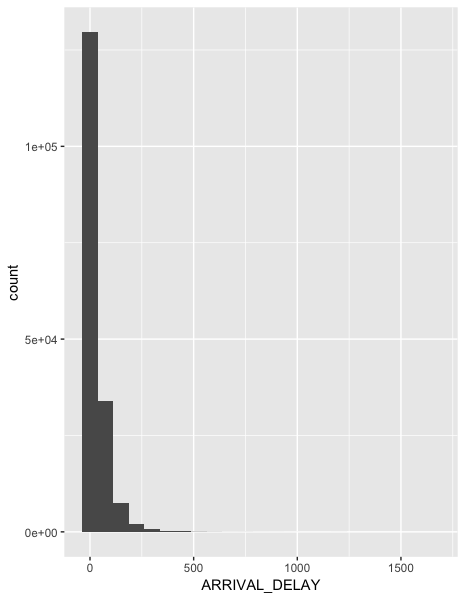
\includegraphics{/Users/rhino/project_proposal/hist.png}
\caption{Delay by flight hour}
\end{figure}

\paragraph{Probability of having a
delay}\label{probability-of-having-a-delay}

The first data point I wanted to look at was percentage of flights that
are late (delayed) upon arrival. Initially, I thought this would be
10-15\%. However, according the data that I looked at, around 37.4\% of
flights are delayed - over 150\% higher than I expected! A slightly
higher number of flights were delayed for Departure. Departing flights
were delayed around 39\% of the time for the sample I looked at.

At a rate of 37.4\%, a person would have the following expected chances
of having a delay: P(delay given n number of flights) = 1-(1-0.374)\^{}5
1 flights - 37.4\% 2 flights - 60.8\% 3 flights - 75.5\% 4 flights -
84.6\% 5 flights - 90.4\%

\paragraph{Probability of delay given an
event}\label{probability-of-delay-given-an-event}

The next data point I looked at was determining the probability of an
arrival delay given that a departure delay occured. P(arrival
delay\textbar{}departure delay) The results were not suprising. When
there was a delay on the departure end of flight, there was likely a
delay on the arrival side. The probability of a delay on arrival give
there was a delay on departure was observed was 71.1\%. Where there was
not a delay on departure, you were only expected to be delayed 16.3\% of
the time. This expected outcome seemed obvious, but I wanted to review
it because it might be a good indicator to use in a regression model.

\paragraph{Probability of delay given hour of
departure}\label{probability-of-delay-given-hour-of-departure}

This statistic is the one of the main themes of my analysis. I expected
that the results for the morning would show a lower probability of
delay. My expectations generally follow what was shown in the data. The
results show that early morning hours, that is 4 or 5 AM, show a lower
expected probablity of delay (\textasciitilde{}25\%) than later in the
day and those hours after midnight (+40\%). Due to the difference in
time vs.~how humans, and subsequently airlines, structure their day, I
plan to create some extra elements for future analysis (morning, midday,
evening, overnight). I believe this makes more sense and this is how
major travel sellers present their products. Additionally, flights after
midnight made up less than 1\% of the data so it may make sense to
eliminate them.

\begin{figure}
\centering
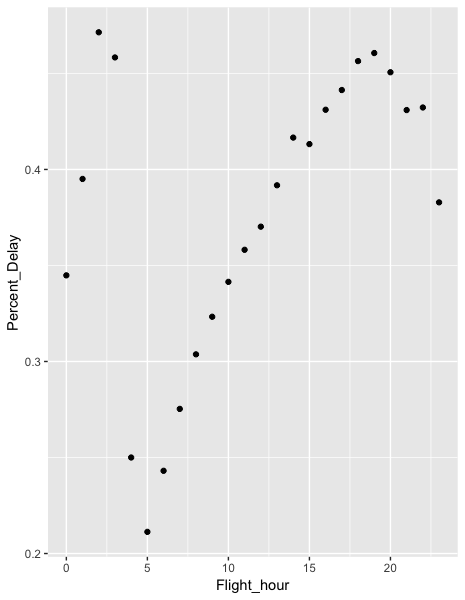
\includegraphics{/Users/rhino/project_proposal/hour.png}
\caption{Delay by flight hour}
\end{figure}

\paragraph{Size of Airport}\label{size-of-airport}

I wanted to see if the size of airport was correlated to the
probablility of a delay. I expected busier airports would have more
delays. However, initial results do not support this idea. It seems that
regardless of size, most of the larger airports seems to hover in the
37\% range according to the graph.

\begin{figure}
\centering
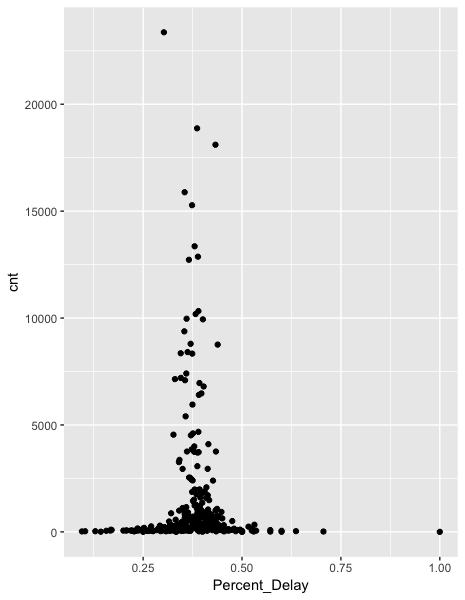
\includegraphics{/Users/rhino/project_proposal/size.png}
\caption{Airport size}
\end{figure}


\end{document}
